\documentclass{article}

\usepackage[T1,T2A]{fontenc}
\usepackage[utf8]{inputenc}
\usepackage[english,russian]{babel}

\usepackage{pdfpages}
\usepackage{multirow}

\usepackage{caption}

\usepackage{amsmath}
\usepackage[hidelinks]{hyperref}


\usepackage{graphicx}%Вставка картинок
\graphicspath{{noiseimages/}}

\usepackage{float}%"Плавающие" картинки
\usepackage{wrapfig}%Обтекание фигур (таблиц, картинок и прочего)

\makeatletter
\def\@biblabel#1{#1. }
\makeatother

\setlength{\emergencystretch}{10pt}

\begin{document}

\begin{table}[ht]
\centering
\begin{tabular}{|c|c|}
\hline
			&Выход по току	\\
\hline
МГД стабильный режим работы &	\\
Момент времени $t_1$			&90.646	\\ 
Момент времени $t_2$		&93.594	\\  
\hline
Выемка 11 и 22 анодов &	\\
Момент времени $t_1$		&89.638	\\  
Момент времени $t_2$		&91.365	\\  
\hline
Анодный эффект &	\\
Момент времени $t_1$	&87.048	\\  
Момент времени $t_2$	&90.037	\\  
\hline
\end{tabular}
\caption{Выход по току $\eta$ для минимального значения МПР ($t_1 < t_2$). \label{table:vichPoToku}}
\end{table}


\begin{table}[ht]
\centering
\begin{tabular}{|c|c|}
\hline
			& Изменение потерь по току (\%)\\
\hline
МГД стабильный режим работы (рис) & 1.038	\\
\hline
Выемка 11 и 22 анодов (рис) &	1.799\\
\hline
Анодный эффект (рис) & 1.262	\\
\hline
\end{tabular}
\caption{Изменение потерь по току. \label{table:ismineniep}}
\end{table}

\begin{figure}[H]
\hspace*{-5cm}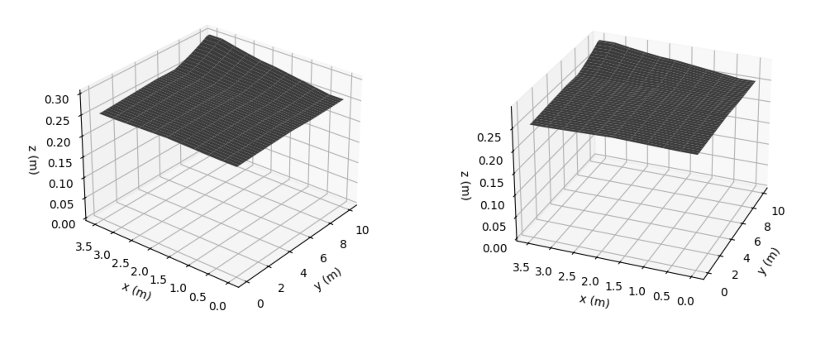
\includegraphics[scale=0.01]{спокойная поверхность.PNG}
\caption{МГД стабильный режим работы}
\end{figure}
\begin{figure}[H]
\hspace*{-5cm}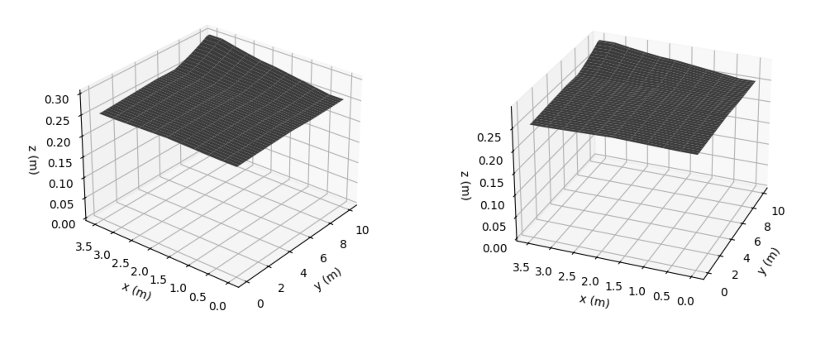
\includegraphics[scale=0.01]{спокойная поверхность.PNG}
\caption{МГД стабильный режим работы}
\end{figure}
\begin{figure}[H]
\hspace*{-5cm}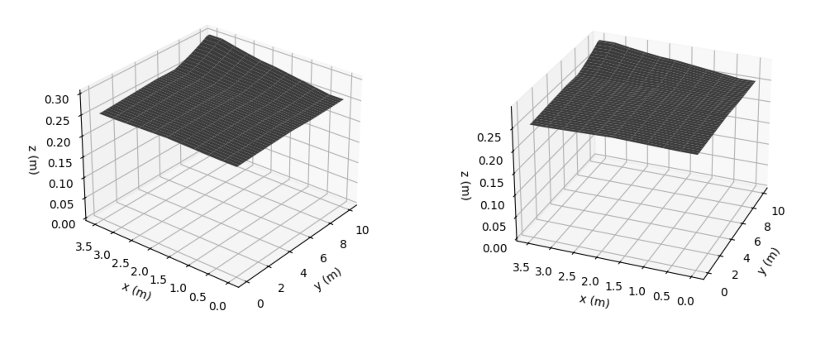
\includegraphics[scale=0.01]{спокойная поверхность.PNG}
\caption{МГД стабильный режим работы}
\end{figure}
\begin{figure}[H]
\hspace*{-5cm}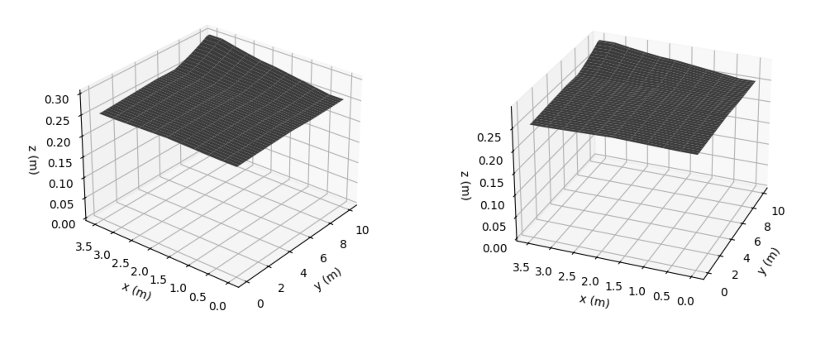
\includegraphics[scale=0.01]{спокойная поверхность.PNG}
\caption{МГД стабильный режим работы}
\end{figure}
\begin{figure}[H]
\hspace*{-5cm}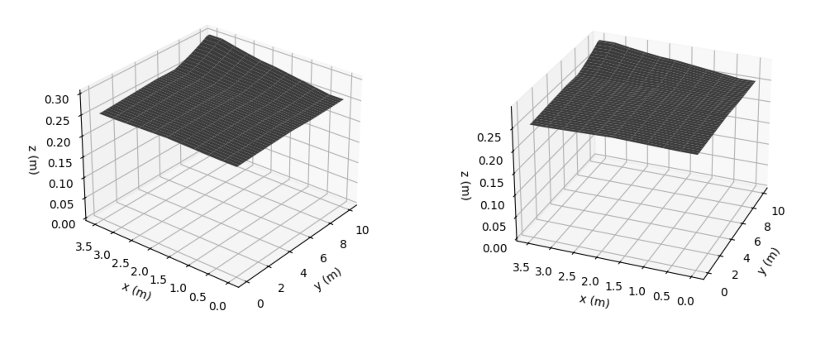
\includegraphics[scale=0.01]{спокойная поверхность.PNG}
\caption{МГД стабильный режим работы}
\end{figure}
\begin{figure}[H]
\hspace*{-5cm}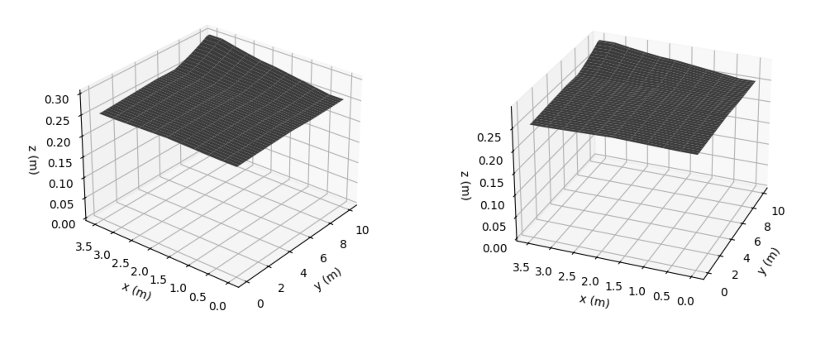
\includegraphics[scale=0.01]{спокойная поверхность.PNG}
\caption{МГД стабильный режим работы}
\end{figure}
\begin{figure}[H]
\hspace*{-5cm}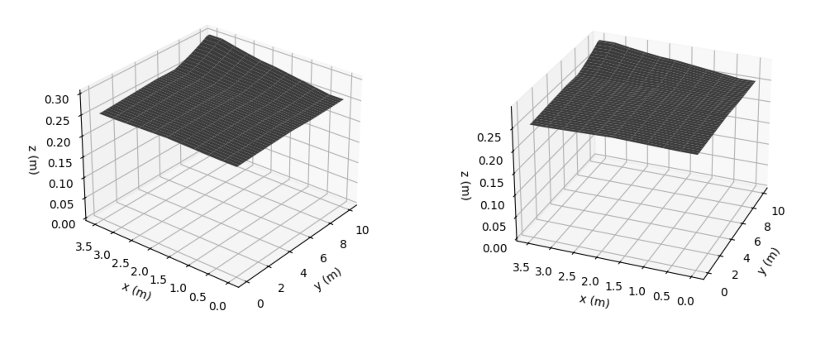
\includegraphics[scale=0.01]{спокойная поверхность.PNG}
\caption{МГД стабильный режим работы}
\end{figure}
\begin{figure}[H]
\hspace*{-5cm}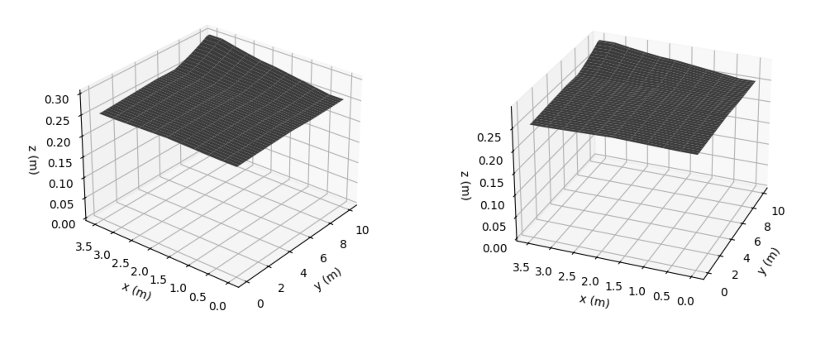
\includegraphics[scale=0.01]{спокойная поверхность.PNG}
\caption{МГД стабильный режим работы}
\end{figure}


\begin{figure}[H]
\hspace*{-4cm}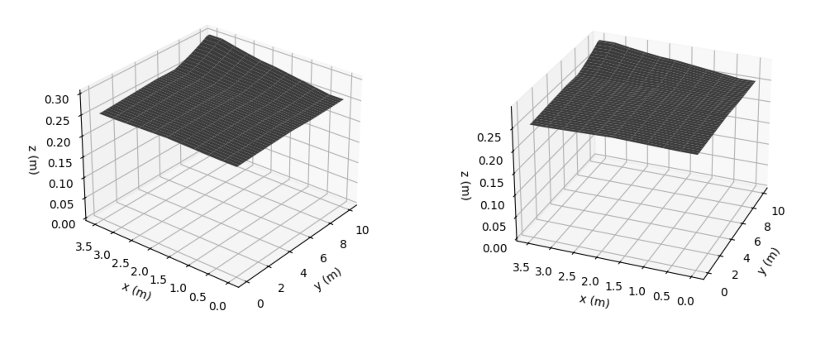
\includegraphics[width=200mm]{спокойная поверхность.PNG}
\caption{МГД стабильный режим работы}
\end{figure}

\begin{figure}[H]
\hspace*{-4cm}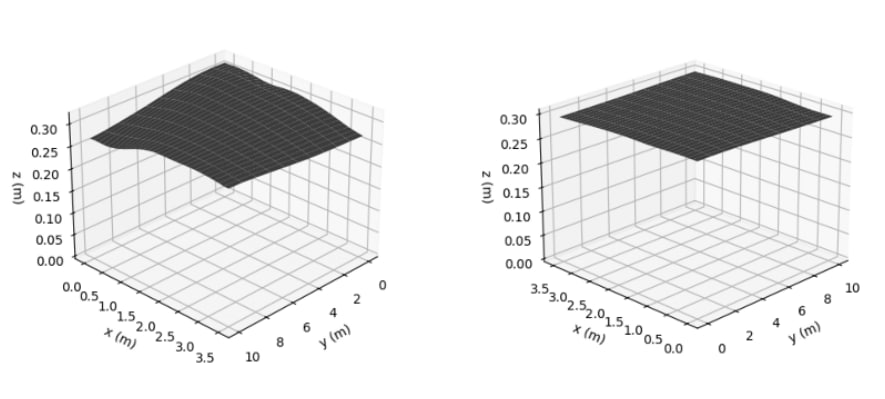
\includegraphics[width=200mm]{Выемка анодов поверхность.PNG}
\caption{Поверхность при выемке анодов}
\end{figure}

\begin{figure}[H]
\hspace*{-4cm}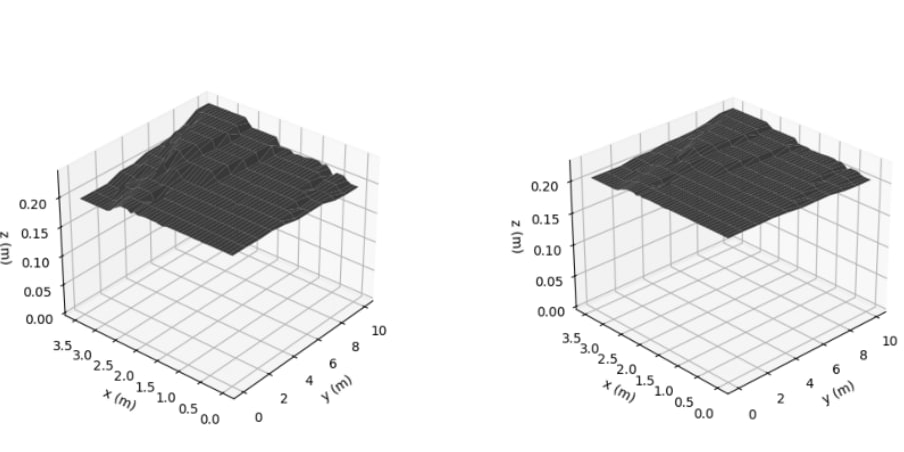
\includegraphics[width=200mm]{Анодный эффект поверхность.PNG}
\caption{Поверхность при анодном эффекте}
\end{figure}

Поскольку формула (6?) представляет из себя поверхностный интеграл, она позволяет получить распределение потерь по току по горизонтальному срезу ванны. Распределение потерь по току наглядно показано на рисунках 12?, 13?, 14? для поверхностей в режимах стабильной работы, МГД нестабильности при выемке анодов и МГД нестабильности при анодном эффекте соответственно. Множитель $\mu = 10^{-6}$.

Измерения МПР проводятся вдоль борта AB, как правило, берется лишь одно измерение посередине ванны. Для МГД-стабильного режима работы ванны и случая выемки анодов такое измерение действительно даст представление о характере происходящих процессах и позволит принять соответствующие меры, однако в случае анодного эффекта результат измерения может сильно варьироваться в зависимости от выбранной точки измерения, что может ввести в заблуждение и привести к увеличению потерь по току или даже выходу электролизера из строя.

\begin{figure}[H]
\hspace*{-5cm}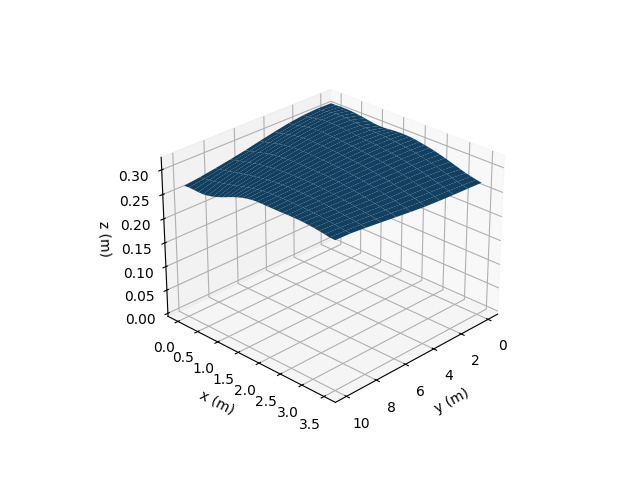
\includegraphics[width=200mm]{h.PNG}
\caption{МГД стабильный режим работы}
\end{figure}

\begin{figure}[H]
\hspace*{-5cm}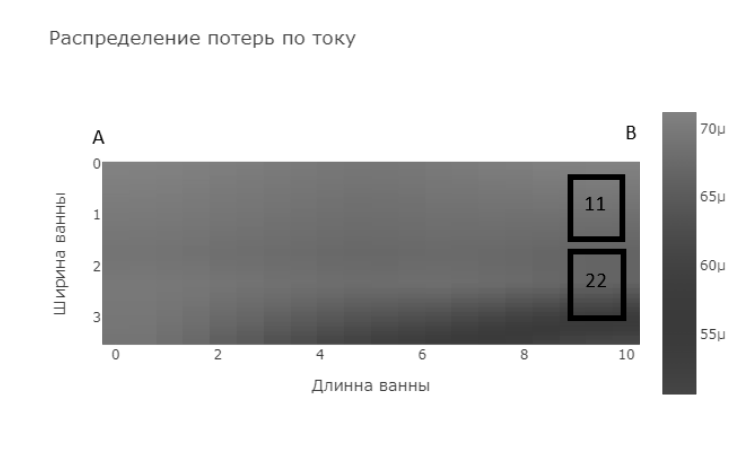
\includegraphics[width=200mm]{выемка анодов.PNG}
\caption{Поверхность при выемке анодов}
\end{figure}

\begin{figure}[H]
\hspace*{-5cm}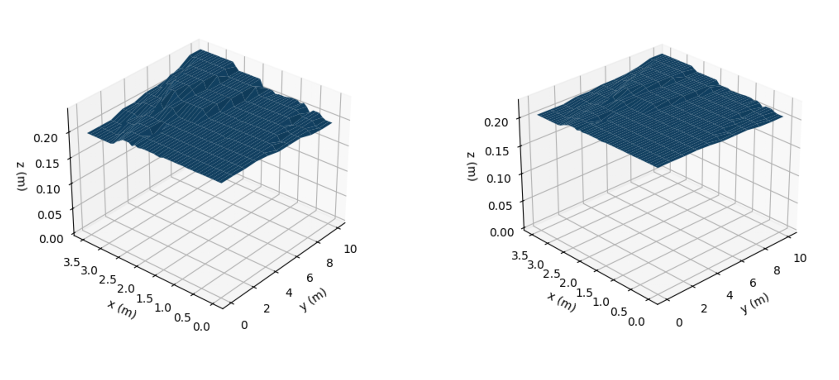
\includegraphics[width=200mm]{анодный эффект.PNG}
\caption{Поверхность при анодном эффекте}
\end{figure}

\end{document}